\documentclass[12pt]{beamer}
\usetheme{Berkeley}
\usepackage[utf8]{inputenc}
\usepackage[german]{babel}
\usepackage[T1]{fontenc}
\usepackage{amsmath}
\usepackage{amsfonts}
\usepackage{amssymb}
\usepackage{graphicx}
\author{Veronica Schier \\ Adrian Löwenberg Casas \\ Julien Caselmann}
\title{Die Kuen'sche Fläche - die schönste Bianchi - Transformation der Pseudosphäre}
%\setbeamercovered{transparent} 
%\setbeamertemplate{navigation symbols}{} 
%\logo{} 
%\institute{} 
%\date{} 
%\subject{} 
\begin{document}

\begin{frame}
\titlepage
\end{frame}

%\begin{frame}
%\tableofcontents
%\end{frame}

\begin{frame}{Parametrisierung}
\begin{center}
$
\begin{pmatrix}
x\\y\\z
\end{pmatrix}
 =
\begin{pmatrix}
\frac{2cosh(u)* \left( cos(v) + v*sin(v) \right)}{v^2+cosh(u)^2}\\\\
\frac{2cosh(u)*(sin(v) - v*cos(v))}{v^2 + cosh(u)^2}\\\\
\frac{sinh(2u)}{v^2 + cosh(u)^2}
\end{pmatrix}
u,v \in \left[ -2\pi , 2\pi \right] $
\end{center}
\end{frame}

\begin{frame}{Ursprung und Entdeckung}
Dieser Typ Kuen. Wie hat er sie gefunden? Was genau hat er gemacht?
Bla bla Bianchi ganz kurz erwähnen
\end{frame}

%Quellen für nächste Folie:
% https://www.mathcurve.com/surfaces.gb/pseudosphere/pseudosphere.shtml
%https://de.wikipedia.org/wiki/Pseudosph%C3%A4re
\begin{frame}{Pseudosphäre}
\begin{enumerate}
\item untersucht von Ferdinand Minding und Eugene Beltrami in 1868
\item auch bekannt als Beltrami-Fläche, Traktroid oder Traktrikoid
\item Pseudosphäre mit Radius $R$ hat konstante, negative Gaußkrümmung $-\frac{1}{R^2}$
\end{enumerate}
\end{frame}

\begin{frame}{Beispiel: Drehfläche einer Traktrix}
Parametrisierung
\end{frame}

\begin{frame}{Beispiel: Drehfläche einer Traktrix}
\begin{center}
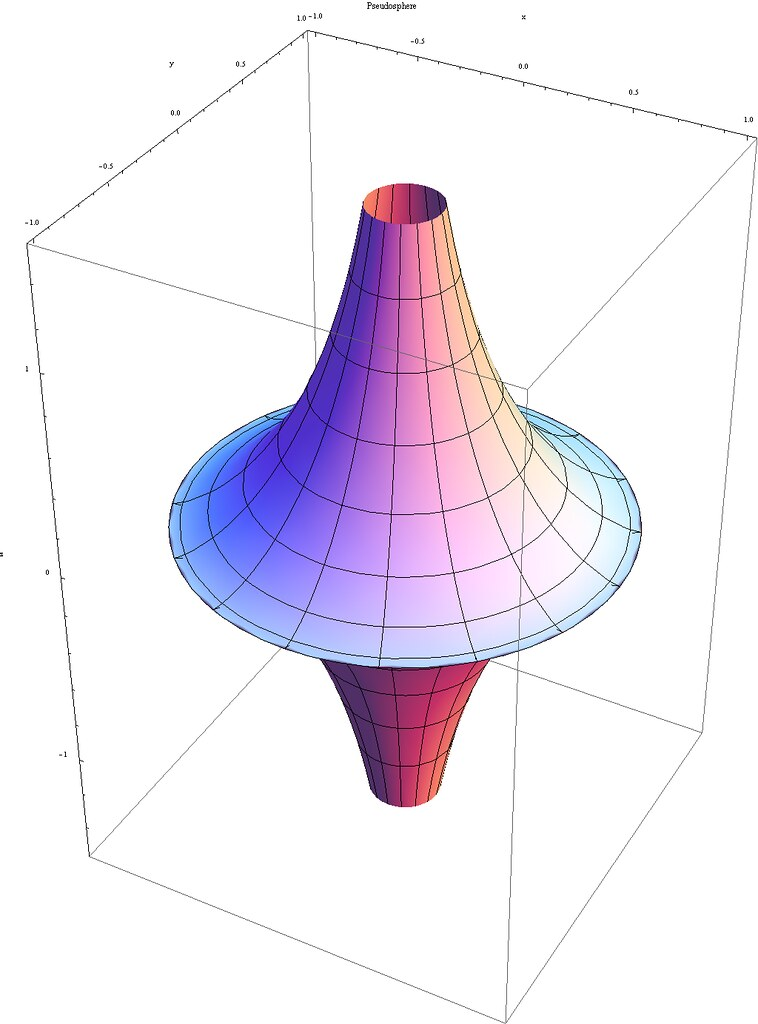
\includegraphics[scale=0.2]{pseudosphere.png}
\end{center}
\end{frame}


\begin{frame}{Bianchi - Transformationen}
\begin{enumerate}
\item behält Gesamtkrümmung bei

\end{enumerate}
\end{frame}

\end{document}